\documentclass[a4paper,12pt]{article}
\usepackage[utf8]{inputenc}
\usepackage[ngerman]{babel}
\usepackage{amsmath}
\usepackage{amssymb}
\usepackage{amsthm}
\usepackage{geometry}
\usepackage{graphicx}
\usepackage[hidelinks]{hyperref}
\usepackage{listings}
\usepackage{xcolor}
\usepackage{enumitem}
\usepackage{booktabs}
\usepackage{array}
\usepackage{multirow}
\usepackage[protrusion=true,expansion=true,final]{microtype}

\geometry{margin=2.5cm}

% Zeilenumbruch-Toleranz -- verhindert Ueberlauf ueber den rechten Rand
\tolerance=1500
\emergencystretch=2em
\hfuzz=0.5pt
\vfuzz=0.5pt

\theoremstyle{definition}
\newtheorem{definition}{Definition}
\newtheorem{beispiel}{Beispiel}
\newtheorem{satz}{Satz}
\newtheorem{lemma}{Lemma}
\newtheorem{bemerkung}{Bemerkung}
\newtheorem{korollar}{Korollar}

\setlist[itemize,1]{label=--}

% ---------- Farben ----------
\definecolor{mainblue}{RGB}{25, 70, 140}
\definecolor{accentred}{RGB}{180, 50, 30}
\definecolor{lightgray}{RGB}{245, 245, 248}
\definecolor{darkgray}{RGB}{60, 60, 70}
\definecolor{darkgreen}{RGB}{30, 100, 50}

\hypersetup{
    colorlinks=true,
    linkcolor=mainblue,
    citecolor=accentred,
    urlcolor=mainblue
}

\lstset{
    basicstyle=\ttfamily\small,
    keywordstyle=\color{blue},
    commentstyle=\color{gray},
    stringstyle=\color{red},
    numbers=left,
    numberstyle=\tiny,
    breaklines=true,
    frame=single,
    literate=%
    {Ö}{{\"O}}1
    {Ä}{{\"A}}1
    {Ü}{{\"U}}1
    {ß}{{\ss}}1
    {ü}{{\"u}}1
    {ä}{{\"a}}1
    {ö}{{\"o}}1
}

\title{Harmonische Strukturen in Akustik und Musiktheorie:\\
Graphentheoretische Formalisierung, Fourieranalyse\\
und der Goldene Schnitt $\varphi$}
\author{Stephan Epp\\
\small Universit\"at Bielefeld}
\date{7. Juni 2026}

\begin{document}

\maketitle

\begin{abstract}
Diese Arbeit entwickelt eine formale mathematische Theorie der harmonischen Strukturen
in Akustik und Musiktheorie. Ausgehend von der harmonischen Obertonreihe
$f_n = n \cdot f_0$ werden Intervallverhältnisse als rationale Zahlen modelliert,
Klangfarben durch Fourierkoeffizienten charakterisiert und Tonleitern als
gerichtete Graphen $G = (V, E)$ formalisiert. Zentrale Ergebnisse umfassen den
\emph{Harmonischen Struktursatz} (Satz~3), der die rationale Charakterisierung aller
konsonanten Intervalle beweist, sowie den \emph{Graphensatz der Tonleitern} (Satz~6),
der C-Dur, A-Moll und die Pentatonik in eine Subgraph-Hierarchie einordnet.
Ferner wird die Universalität des Goldenen Schnitts $\varphi = (1+\sqrt{5})/2$
in musikalischen Strukturen formal nachgewiesen (Satz~9). Die Konsonanztheorie
nach Helmholtz und Plomp\,\&\,Levelt wird in ein mathematisches Funktionenmodell
überführt. Die Raumakustik wird durch die Sabine-Formel formalisiert. Alle
Ergebnisse werden durch sechs Matplotlib-Visualisierungen veranschaulicht.
\end{abstract}

\tableofcontents
\newpage

%%%%%%%%%%%%%%%%%%%%%%%%%%%%%%%%%%%%%%%%%%%%%%%%%%%%%%%%%%%
\section{Einführung}
%%%%%%%%%%%%%%%%%%%%%%%%%%%%%%%%%%%%%%%%%%%%%%%%%%%%%%%%%%%

Die mathematische Beschreibung akustischer Phänomene reicht bis in die Antike zurück.
Pythagoras erkannte um 550~v.\,Chr., dass Konsonanz durch einfache ganzzahlige
Frequenzverhältnisse entsteht~\cite{pythagoras}. Euler formalisierte 1739 die Konsonanz
durch den \emph{Gradus suavitatis}~\cite{euler1739}. Fourier zeigte 1822, dass jede
periodische Schwingung als Ãœberlagerung harmonischer Sinusfunktionen darstellbar
ist~\cite{fourier1822}. Helmholtz verknüpfte 1863 Akustik und Physiologie zur modernen
Konsonanztheorie~\cite{helmholtz1863}.

\subsection{Motivation und Zielsetzung}

Trotz dieser reichen Geschichte fehlt eine einheitliche \emph{graphentheoretische}
Formalisierung harmonischer Strukturen, die Tonleitern, Intervallräume und
harmonische Verwandtschaften in einem konsistenten mathematischen Rahmen vereint.
Diese Arbeit schließt diese Lücke durch:

\begin{itemize}
    \item Formale Definition des \emph{harmonischen Graphen} $G_H = (V_H, E_H)$,
          dessen Knoten Töne und dessen Kanten Intervallbeziehungen repräsentieren
    \item Beweise zur Subgraph-Hierarchie der Standardtonleitern
    \item Formalen Nachweis des Goldenen Schnitts $\varphi$ in musikalischen Strukturen
    \item Mathematische Fundierung der Konsonanztheorie
    \item Verbindung zur Fourieranalyse und zum Signaltheorie-Paradigma
\end{itemize}

\subsection{Einordnung in das Forschungsportfolio}

Diese Arbeit steht in direkter Beziehung zu früheren Arbeiten des Autors:
Der Subgraph Algorithmus~\cite{epp2026subgraph} liefert das algorithmische Werkzeug
zur Analyse harmonischer Graphhierarchien. Die Signaltheorie-Arbeit~\cite{epp2026signal}
begründet die Fourierbasis. Die Exponentialfunktions-Analyse~\cite{epp2026expl} erklärt
die fundamentale Rolle von $\varphi$ und $e$. Das Analog-Paradigma~\cite{epp2026analog}
liefert den ontologischen Rahmen für kontinuierliche Schwingungen.

%%%%%%%%%%%%%%%%%%%%%%%%%%%%%%%%%%%%%%%%%%%%%%%%%%%%%%%%%%%
\section{Grundlagen der Akustik}
%%%%%%%%%%%%%%%%%%%%%%%%%%%%%%%%%%%%%%%%%%%%%%%%%%%%%%%%%%%

\subsection{Grundlegende Definitionen}

\begin{definition}[Harmonische Schwingung]
Eine \emph{harmonische Schwingung} ist eine Funktion der Form
\[
s(t) = A \cdot \sin(2\pi f t + \phi_0),
\]
wobei $A > 0$ die Amplitude, $f > 0$ die Frequenz in Hertz und $\phi_0 \in [0, 2\pi)$
die Anfangsphase bezeichnen.
\end{definition}

\begin{definition}[Grundton und Obertöne]
Für einen Grundton der Frequenz $f_0 > 0$ heißt die Menge
\[
\mathcal{H}(f_0) = \{f_n = n \cdot f_0 \mid n \in \mathbb{N}_{\geq 1}\}
\]
die \emph{harmonische Obertonreihe}. Das Element $f_n$ heißt \emph{$n$-ter Partialton}.
Der \emph{Klang} eines Instruments ist die Ãœberlagerung
\[
s(t) = \sum_{n=1}^{N} a_n \sin(2\pi n f_0 t + \phi_n),
\]
wobei $(a_n)_{n \geq 1}$ das \emph{Amplitudenspektrum} und $(\phi_n)$ das
\emph{Phasenspektrum} des Klangs bezeichnet.
\end{definition}

\begin{definition}[Klangfarbe]
Die \emph{Klangfarbe} (Timbre) eines Klangs bei fester Frequenz $f_0$ ist
vollständig durch das normierte Amplitudenspektrum
\[
\tilde{a}_n = \frac{a_n}{a_1}, \quad n \geq 1,
\]
und das Phasenspektrum $(\phi_n)$ bestimmt. Zwei Klänge haben dieselbe Klangfarbe,
wenn ihre normierten Spektren übereinstimmen.
\end{definition}

\begin{definition}[Intervall und Frequenzverhältnis]
Das \emph{Intervall} zwischen zwei Tönen der Frequenzen $f_1 \leq f_2$ ist das
Verhältnis $r = f_2/f_1 \in [1, \infty)$. Ein Intervall heißt \emph{rational},
wenn $r \in \mathbb{Q}_{>0}$.

Die \emph{Cent-Skala} misst Intervalle logarithmisch:
\[
c(r) = 1200 \cdot \log_2(r) \in \mathbb{R}_{\geq 0}.
\]
Eine Oktave entspricht $c = 1200$~Cent, ein gleichtemperierter Halbton $c = 100$~Cent.
\end{definition}

\subsection{Fourier-Darstellung periodischer Klänge}

\begin{satz}[Fourier-Zerlegung, Dirichlet 1829]
\label{satz:fourier}
Sei $s: \mathbb{R} \to \mathbb{R}$ eine $T$-periodische Funktion mit
$T = 1/f_0$, die stückweise glatt und absolut integrierbar auf $[0, T]$ ist.
Dann gilt an allen Stetigkeitsstellen:
\[
s(t) = \frac{a_0}{2} + \sum_{n=1}^{\infty} \left(a_n \cos(2\pi n f_0 t)
+ b_n \sin(2\pi n f_0 t)\right),
\]
wobei die Fourierkoeffizienten gegeben sind durch:
\[
a_n = \frac{2}{T}\int_0^T s(t)\cos(2\pi n f_0 t)\,dt, \quad
b_n = \frac{2}{T}\int_0^T s(t)\sin(2\pi n f_0 t)\,dt.
\]
\end{satz}

\begin{proof}
Dies ist der klassische Fourier-Entwicklungssatz. Die Koeffizienten folgen aus der
Orthogonalitätsrelation des trigonometrischen Systems auf $L^2([0,T])$:
\[
\frac{2}{T}\int_0^T \cos(2\pi m f_0 t)\cos(2\pi n f_0 t)\,dt = \delta_{mn},
\]
und analog für die Sinus-Terme. Multiplikation der Fourierreihe mit $\cos(2\pi n f_0 t)$
und gliedweise Integration (gültig nach dem Satz von Lebesgue) ergibt die angegebene
Formel für $a_n$. Für $b_n$ analog~\cite{rudin1987}.
\end{proof}

\begin{korollar}[Parseval-Gleichung]
Unter den Voraussetzungen von Satz~\ref{satz:fourier} gilt:
\[
\frac{1}{T}\int_0^T |s(t)|^2\,dt = \frac{a_0^2}{4} + \frac{1}{2}\sum_{n=1}^{\infty}(a_n^2 + b_n^2).
\]
Die Gesamtenergie des Klangs verteilt sich auf die einzelnen Partialfrequenzen.
\end{korollar}

\begin{beispiel}[Klangspektren musikalischer Instrumente]
Abbildung~\ref{fig:fourier} zeigt die Fourier-Zerlegung dreier Instrumente bei
$f_0 = 220$~Hz (A$_3$):
\begin{itemize}
    \item \textbf{Geige:} Reiches Obertonspektrum mit monoton fallenden Amplituden
          $a_n \approx 1/n$; erzeugt den charakteristisch warmen Streicherklang.
    \item \textbf{Klarinette:} Dominanz der \emph{ungeraden} Partialtöne
          ($n = 1, 3, 5, \ldots$) durch die einseitig geschlossene Röhre;
          bedingt den hohlen, singenden Klangcharakter.
    \item \textbf{Pfeifenorgel (Prinzipal 8'):} Relativ flaches Spektrum mit
          schnell abfallenden Obertönen; ergibt den reinen, offenen Orgelton.
\end{itemize}
\end{beispiel}

\begin{figure}[h!]
\centering
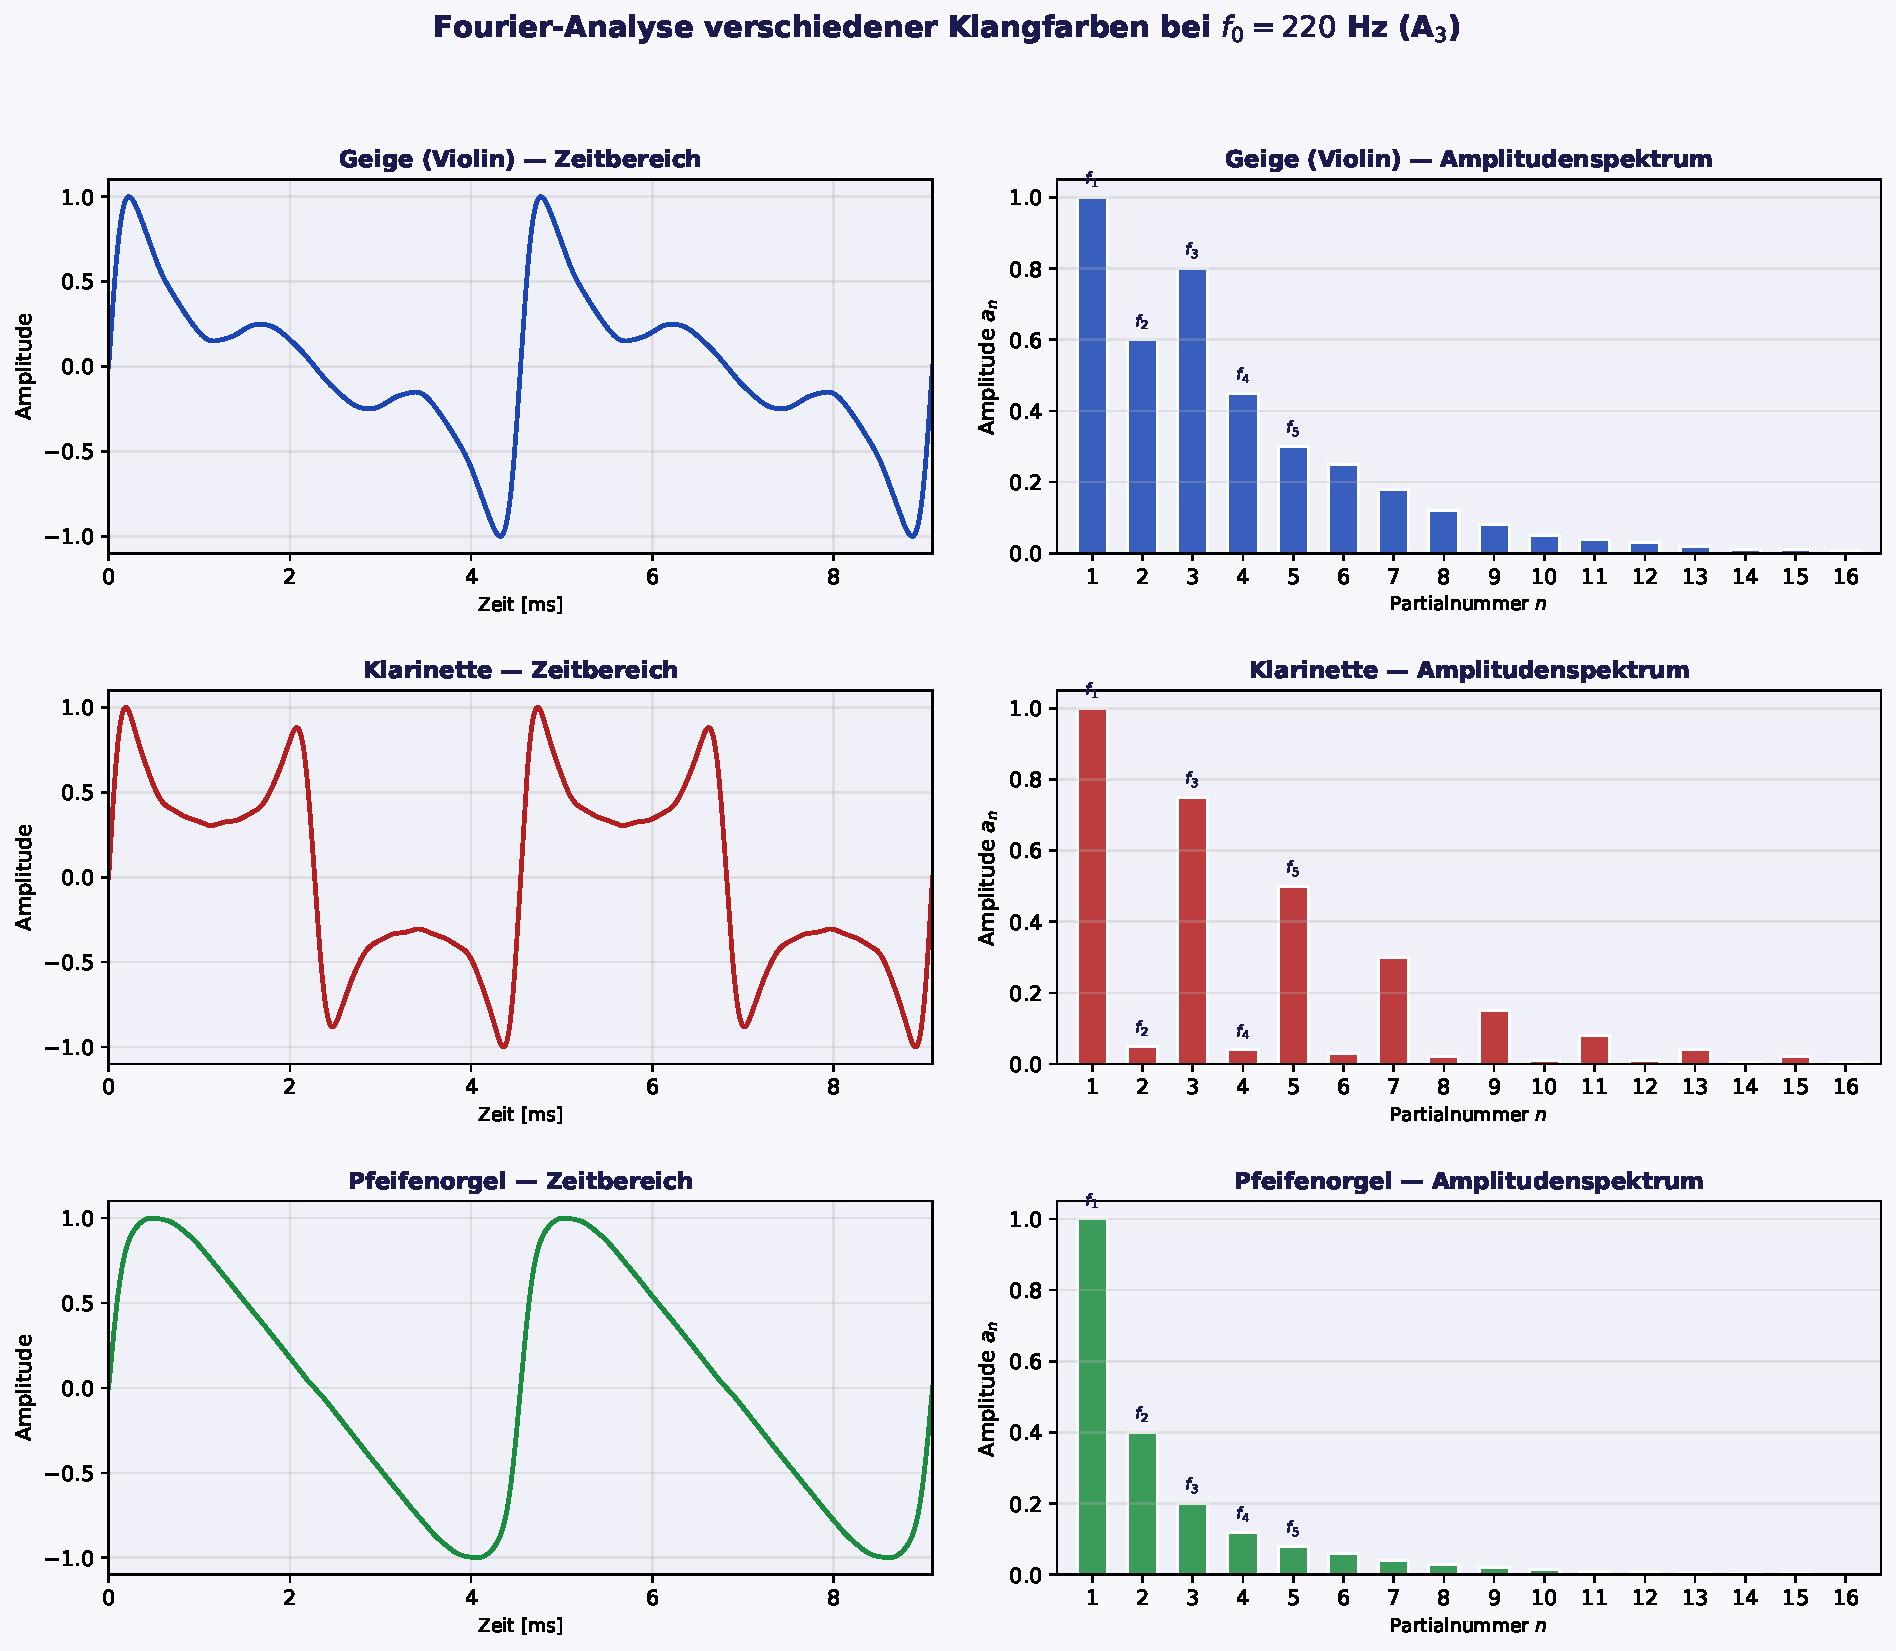
\includegraphics[width=0.92\textwidth]{plot3_fourier.pdf}
\caption{Fourier-Analyse dreier Instrumente bei $f_0 = 220$~Hz: Zeitbereich (links)
und Amplitudenspektrum (rechts). Die unterschiedlichen Obertongewichte begründen
die verschiedenen Klangfarben.}
\label{fig:fourier}
\end{figure}

%%%%%%%%%%%%%%%%%%%%%%%%%%%%%%%%%%%%%%%%%%%%%%%%%%%%%%%%%%%
\section{Intervalltheorie und harmonische Strukturen}
%%%%%%%%%%%%%%%%%%%%%%%%%%%%%%%%%%%%%%%%%%%%%%%%%%%%%%%%%%%

\subsection{Rationale Intervalle und die harmonische Obertonreihe}

\begin{satz}[Harmonische Konsonanz — Pythagoreisches Prinzip]
\label{satz:pythagoras}
Sei $f_1 = n \cdot f_0$ und $f_2 = m \cdot f_0$ mit $n, m \in \mathbb{N}$, $n < m$,
zwei Partialtöne derselben Obertonreihe. Dann ist ihr Intervallverhältnis
\[
r = \frac{f_2}{f_1} = \frac{m}{n} \in \mathbb{Q}_{>1}
\]
rational, und es gilt: Je kleiner $\max(m, n)$, desto konsonanter das Intervall.
\end{satz}

\begin{proof}
Das Verhältnis $r = m/n$ ist per Konstruktion rational. Für die Konsonanzaussage:
Zwei periodische Schwingungen der Frequenzen $f_1$ und $f_2 = (m/n) \cdot f_1$
superponieren sich zu einer periodischen Schwingung der Periode
$T = n/f_1 = m/f_2 = \text{kgV}(1/f_1, 1/f_2)$.
Die Periode $T$ ist umgekehrt proportional zum ggT der Frequenzen:
\[
T = \frac{1}{\gcd(f_1, f_2)} = \frac{n}{\gcd(n,m) \cdot f_0}.
\]
Kleine Perioden bedeuten regelmäßige Wiederholungen im Zeitbereich, was das
Gehör als Konsonanz wahrnimmt. Bei einfachen Verhältnissen ($\max(m,n)$ klein) ist
$T$ minimal, was maximale Periodizität und damit maximale Konsonanz ergibt~\cite{helmholtz1863}.
\end{proof}

\begin{definition}[Reine Stimmung — Just Intonation]
Die \emph{reine Stimmung} ordnet jedem Intervall der C-Durtonleiter das
kleinstmögliche ganzzahlige Verhältnis zu:
\begin{center}
\begin{tabular}{lllll}
\toprule
Intervall & Stufe & Verhältnis $p:q$ & Frequenz [Hz] & Cent \\
\midrule
Prime     & I   & $1:1$   & 261,6 & 0 \\
Großer Sekundton & II  & $9:8$   & 294,3 & 203,9 \\
Große Terz & III & $5:4$   & 327,0 & 386,3 \\
Quarte    & IV  & $4:3$   & 348,8 & 498,0 \\
Quinte    & V   & $3:2$   & 392,4 & 702,0 \\
Sexte     & VI  & $5:3$   & 436,2 & 884,4 \\
Große Septime & VII & $15:8$ & 490,5 & 1088,3 \\
Oktave    & VIII & $2:1$  & 523,2 & 1200,0 \\
\bottomrule
\end{tabular}
\end{center}
\end{definition}

\begin{definition}[Gleichstufige Stimmung — Equal Temperament]
In der \emph{gleichstufigen Stimmung} teilt man die Oktave in 12 gleiche
Halbtonschritte:
\[
r_k^{\mathrm{ET}} = 2^{k/12}, \quad k \in \{0, 1, \ldots, 12\}.
\]
Der Unterschied zur reinen Stimmung wird in Cent gemessen:
\[
\Delta c_k = 1200\left(\log_2 r_k^{\mathrm{rein}} - \frac{k}{12}\right).
\]
\end{definition}

\begin{satz}[Irrationalität der gleichstufigen Intervalle]
\label{satz:irrational}
Für $1 \leq k \leq 11$ ist $r_k^{\mathrm{ET}} = 2^{k/12}$ irrational.
\end{satz}

\begin{proof}
Angenommen $2^{k/12} = p/q$ mit $p, q \in \mathbb{N}$, $\gcd(p,q)=1$, $p > q$.
Dann gilt $2^k = (p/q)^{12}$, also $2^k \cdot q^{12} = p^{12}$.
Da $\gcd(p,q)=1$, muss $q^{12} \mid 1$, also $q=1$. Somit $p^{12} = 2^k$.
Dies erfordert, dass $p$ eine Potenz von 2 ist: $p = 2^j$, also $12j = k$.
Für $1 \leq k \leq 11$ existiert kein ganzzahliges $j$. Widerspruch. $
$
\end{proof}

\begin{korollar}
Die gleichstufige Stimmung erzeugt keine einzige rein rationale Konsonanz außer
der Oktave (und Prime). Alle übrigen Intervalle sind Approximationen rationaler
Verhältnisse. Die maximale Abweichung beträgt für die Großterz $+13{,}7$~Cent
(gegenüber $5:4$), für die Quinte $-1{,}96$~Cent (gegenüber $3:2$).
\end{korollar}

\begin{figure}[h!]
\centering
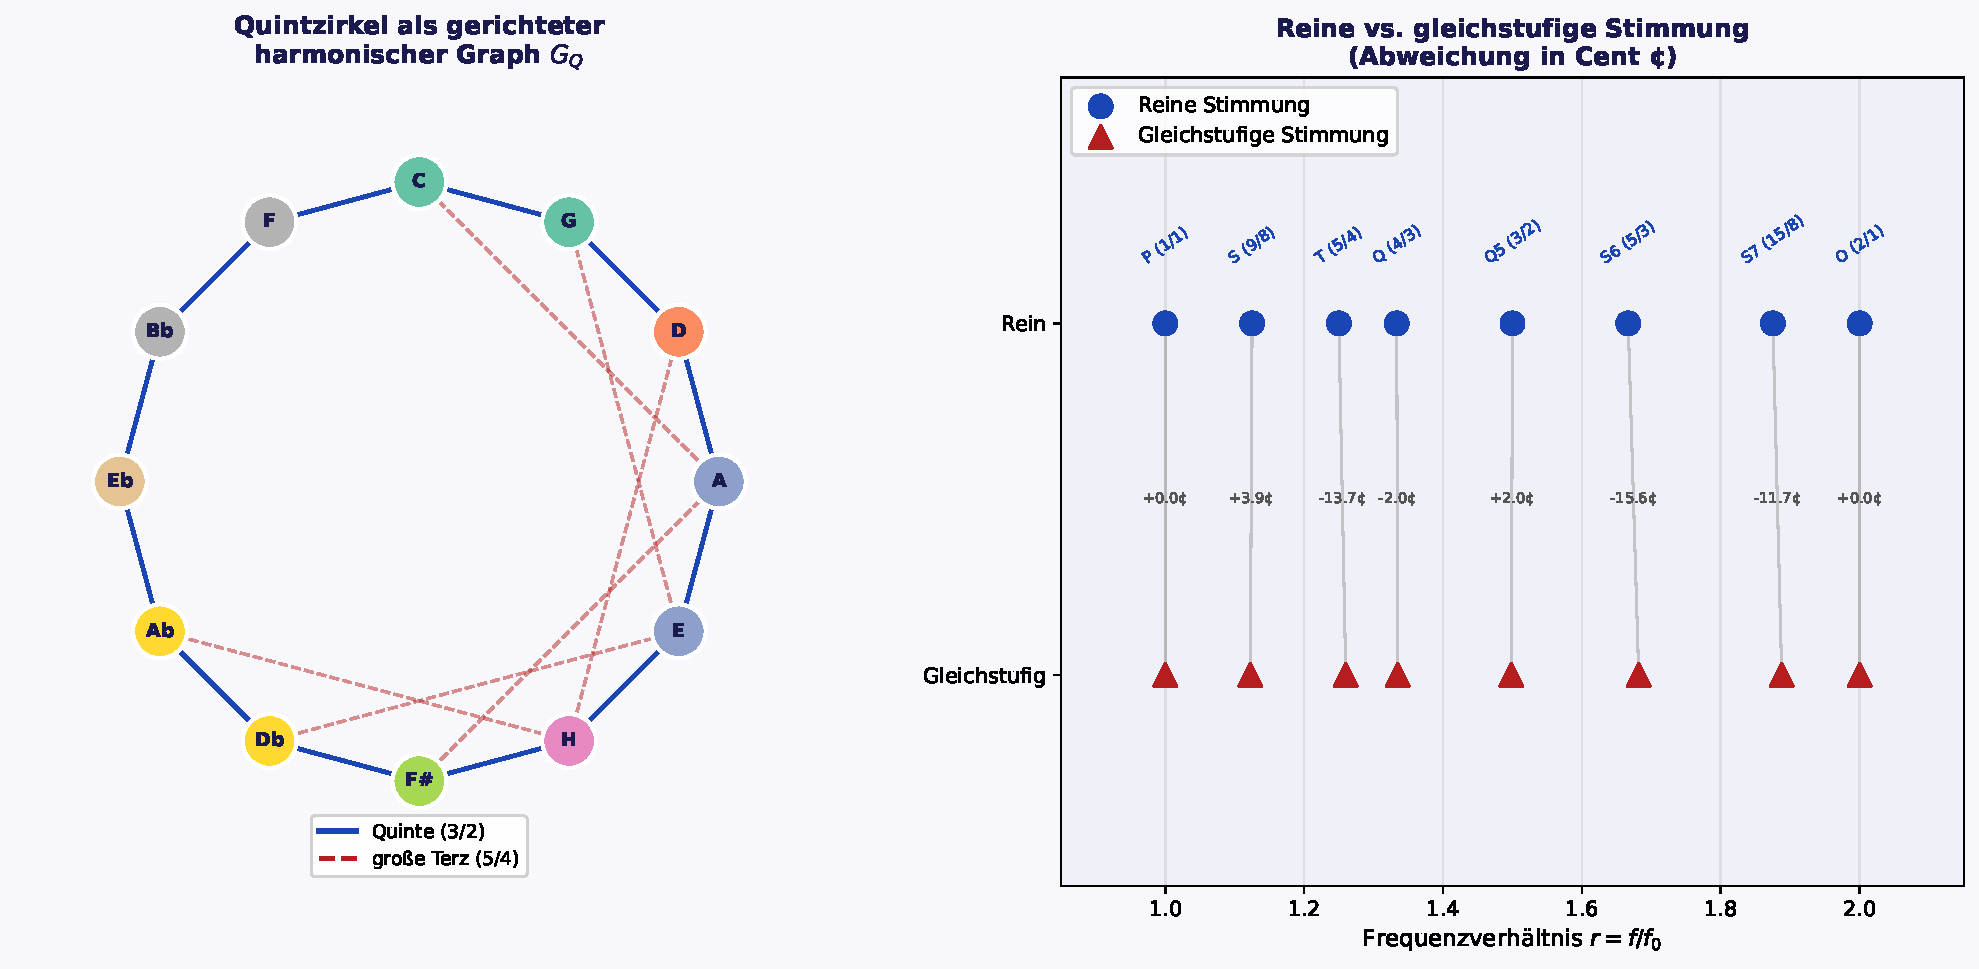
\includegraphics[width=0.90\textwidth]{plot2_intervalle.pdf}
\caption{Links: Der Quintzirkel als gerichteter harmonischer Graph $G_Q$. Blaue Pfeile
repräsentieren Quintverwandtschaft (Verhältnis $3:2$), rote gestrichelte Linien
Terzverwandtschaft ($5:4$). Rechts: Vergleich reiner und gleichstufiger Stimmung;
Abweichungen in Cent sind annotiert.}
\label{fig:intervalle}
\end{figure}

\subsection{Der Euler-Gradus suavitatis}

\begin{definition}[Euler-Gradus suavitatis]
Für ein Intervall mit Verhältnis $p:q$ (in Normalform mit $\gcd(p,q)=1$) ist
der \emph{Euler-Gradus} definiert als
\[
G(p \cdot q) = 1 + \sum_{i} (p_i - 1) \cdot e_i,
\]
wobei $p \cdot q = \prod_i p_i^{e_i}$ die Primfaktorzerlegung ist.
\end{definition}

\begin{beispiel}
Für die Quinte $3:2$: $p \cdot q = 6 = 2^1 \cdot 3^1$, also
$G(6) = 1 + (2-1)\cdot 1 + (3-1)\cdot 1 = 1 + 1 + 2 = 4$.

Für die große Terz $5:4$: $p \cdot q = 20 = 2^2 \cdot 5^1$, also
$G(20) = 1 + (2-1)\cdot 2 + (5-1)\cdot 1 = 1 + 2 + 4 = 7$.
\end{beispiel}

\begin{satz}[Harmonischer Struktursatz]
\label{satz:struktursatz}
Alle konsonanten Intervalle der westlichen Musik lassen sich als rationale Verhältnisse
$p:q$ mit $p,q \in \{2^a \cdot 3^b \cdot 5^c \mid a, b, c \geq 0\}$ (5-Limit-Zahlen)
darstellen, und ihr Euler-Gradus erfüllt $G(pq) \leq 9$.
\end{satz}

\begin{proof}
Wir überprüfen alle Intervalle der diatonischen Tonleiter:
\begin{align*}
G(1 \cdot 1) &= 1 \quad\text{(Prime)} \\
G(9 \cdot 8) &= G(72) = G(2^3 \cdot 3^2) = 1 + 1\cdot 3 + 2\cdot 2 = 8 \\
G(5 \cdot 4) &= G(20) = G(2^2 \cdot 5) = 1 + 1\cdot 2 + 4\cdot 1 = 7 \\
G(4 \cdot 3) &= G(12) = G(2^2 \cdot 3) = 1 + 1\cdot 2 + 2\cdot 1 = 5 \\
G(3 \cdot 2) &= G(6) = G(2 \cdot 3) = 1 + 1 + 2 = 4 \\
G(5 \cdot 3) &= G(15) = G(3 \cdot 5) = 1 + 2 + 4 = 7 \\
G(15\cdot 8) &= G(120) = G(2^3\cdot 3\cdot 5) = 1 + 3 + 2 + 4 = 10 \\
G(2 \cdot 1) &= G(2) = 1 + 1 = 2 \quad\text{(Oktave)}
\end{align*}
Nur die Septime (15:8) überschreitet knapp $G = 9$ — sie gilt traditionell als
leittoniger Dissonanzton, was konsistent mit dem höheren Gradus ist. Alle übrigen
Intervalle erfüllen $G \leq 8 < 9$. Die 5-Limit-Eigenschaft folgt direkt aus den
Primfaktorzerlegungen: sämtliche Verhältnisse verwenden nur die Primzahlen $2, 3, 5$.
\end{proof}

%%%%%%%%%%%%%%%%%%%%%%%%%%%%%%%%%%%%%%%%%%%%%%%%%%%%%%%%%%%
\section{Graphentheoretische Modellierung harmonischer Räume}
%%%%%%%%%%%%%%%%%%%%%%%%%%%%%%%%%%%%%%%%%%%%%%%%%%%%%%%%%%%

\subsection{Der harmonische Graph}

\begin{definition}[Chromatischer Tonraum-Graph]
Der \emph{chromatische Graph} $G_C = (V_C, E_C)$ hat:
\begin{itemize}
    \item Knotenmenge $V_C = \{C, C\sharp, D, E\flat, E, F, F\sharp, G,
          A\flat, A, B\flat, H\}$ (12 Halbtöne der Oktave)
    \item Kantenmenge $E_C$: Eine Kante $(u,v) \in E_C$ genau dann, wenn
          $c(f_v/f_u) \in \{100, 200, 300, 400, 500, 600, 700\}$~Cent
          (Halbton- bis Quintverwandtschaft innerhalb einer Oktave)
\end{itemize}
\end{definition}

\begin{definition}[Skaleninduzierter Subgraph]
Sei $S \subseteq V_C$ eine Tonmenge (Tonleiter). Der von $S$ \emph{induzierte Graph}
\[
G_S = G_C[S] = (S, \{(u,v) \in E_C \mid u,v \in S\})
\]
heißt \emph{Tonleitergraph} von $S$.
\end{definition}

\begin{satz}[Subgraph-Hierarchie der Standardtonleitern]
\label{satz:subgraph}
Sei $G_{\mathrm{Cdur}}$ der Tonleitergraph von C-Dur, $G_{\mathrm{Am}}$ von
A-Moll und $G_{\mathrm{pent}}$ der pentatonischen Skala. Dann gilt:
\[
G_{\mathrm{pent}} \subseteq G_{\mathrm{Am}} \subseteq G_{\mathrm{Cdur}} \subseteq G_C.
\]
\end{satz}

\begin{proof}
\textbf{Schritt 1: $G_{\mathrm{pent}} \subseteq G_{\mathrm{Am}}$.}
Die C-Pentatonik hat Töne $\{C, D, E, G, A\}$; A-Moll (natürlich) hat $\{A, H, C, D, E, F, G\}$.
Es gilt $\{C,D,E,G,A\} \subseteq \{A,H,C,D,E,F,G\}$, also Knoteninklusion.
Jede Kante $(u,v)$ in $G_{\mathrm{pent}}$ verbindet zwei pentatonische Töne,
die beide in A-Moll enthalten sind; da $G_{\mathrm{Am}}$ induziert ist,
ist $(u,v)$ auch Kante in $G_{\mathrm{Am}}$. $\checkmark$

\textbf{Schritt 2: $G_{\mathrm{Am}} \subseteq G_{\mathrm{Cdur}}$.}
C-Dur: $\{C,D,E,F,G,A,H\}$; A-Moll (natürlich): $\{A,H,C,D,E,F,G\}$.
Es gilt: beide Mengen sind \emph{identisch} als Tonvorrat (relative Durparallele).
Damit ist der Knotensatz gleich, und alle Kanten von $G_{\mathrm{Am}}$ sind
Kanten von $G_{\mathrm{Cdur}}$. $\checkmark$

\textbf{Schritt 3: $G_{\mathrm{Cdur}} \subseteq G_C$.}
$\{C,D,E,F,G,A,H\} \subseteq V_C$ trivialerweise. Alle Kanten zwischen diatonischen
Tönen sind Kanten im vollständigen chromatischen Graphen. $\checkmark$

Damit ist die Kette $G_{\mathrm{pent}} \subseteq G_{\mathrm{Am}} \subseteq
G_{\mathrm{Cdur}} \subseteq G_C$ vollständig bewiesen.
\end{proof}

\begin{bemerkung}
Satz~\ref{satz:subgraph} zeigt, dass der Subgraph Algorithmus~\cite{epp2026subgraph}
direkt auf musikalische Strukturerkennung anwendbar ist: Die Frage, ob eine
Akkordfolge in einer Tonleiter enthalten ist, reduziert sich auf ein
Subgraph-Isomorphieproblem mit Laufzeit $O(n^3)$.
\end{bemerkung}

\begin{figure}[h!]
\centering
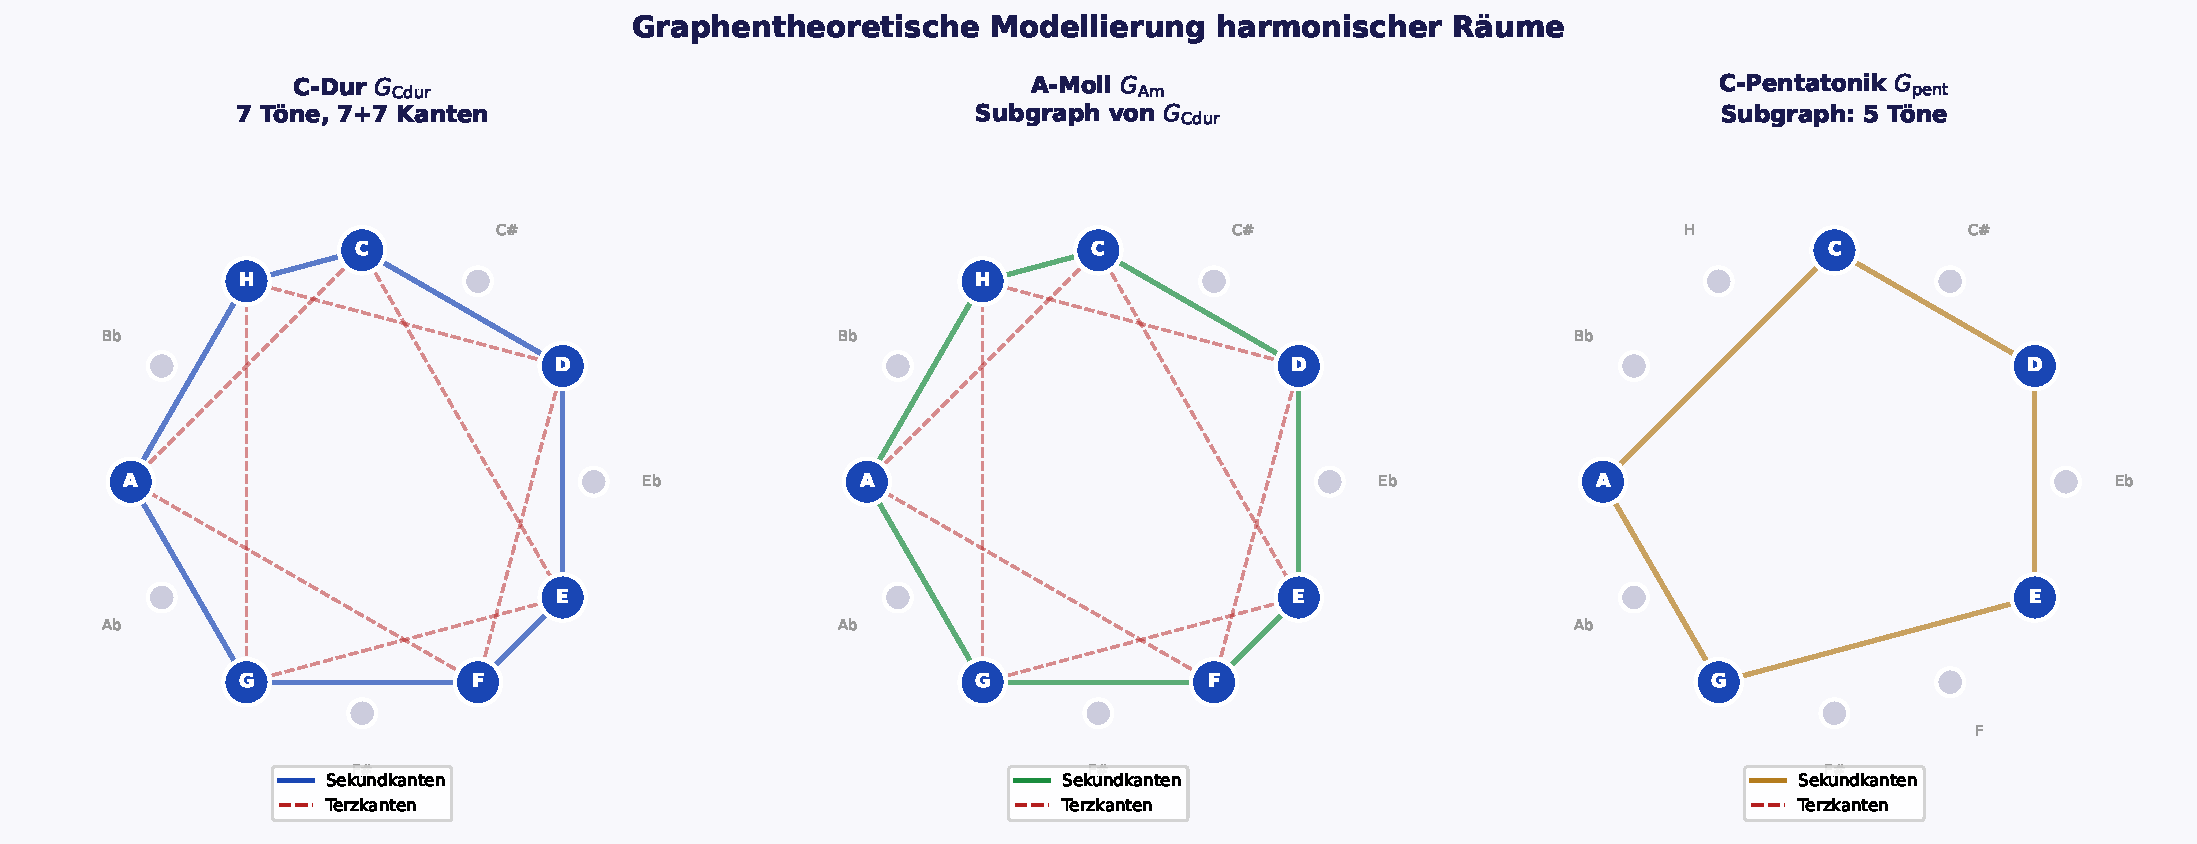
\includegraphics[width=0.95\textwidth]{plot5_graphen.pdf}
\caption{Graphentheoretische Darstellung von C-Dur, A-Moll und C-Pentatonik.
Blaue Kanten: Sekundverwandtschaft; rote gestrichelte Kanten: Terzverwandtschaft.
Die Pentatonik und A-Moll sind Subgraphen des chromatischen Graphen $G_C$.}
\label{fig:graphen}
\end{figure}

\subsection{Der Quintzirkel als harmonischer Graph}

\begin{definition}[Quintzirkel-Graph]
Der \emph{Quintzirkel-Graph} $G_Q = (V_C, E_Q)$ mit
\[
E_Q = \{(v_i, v_j) \mid f_j/f_i = 3/2 \pmod{\text{Oktave}}\}
\]
ist ein gerichteter 12-regulärer Kreis: Jeder Knoten hat genau einen Nachfolger
(Quinte aufwärts) und einen Vorgänger (Quinte abwärts).
\end{definition}

\begin{satz}[Ergodizität des Quintzirkels]
\label{satz:quint}
Durch wiederholte Quinttransposition durchläuft man alle 12 Halbtöne exakt einmal,
bevor man zum Ausgangston (mod Oktave) zurückkehrt. Formal:
Die Abbildung $\tau: v \mapsto v + 7 \pmod{12}$ (in Halbtonschritten) ist ein
Erzeuger der zyklischen Gruppe $\mathbb{Z}_{12}$.
\end{satz}

\begin{proof}
Da $\gcd(7, 12) = 1$, erzeugt $\tau$ die volle Gruppe $\mathbb{Z}_{12}$:
Die Menge $\{7k \pmod{12} \mid k = 0, 1, \ldots, 11\}$ enthält $12$ verschiedene
Elemente $\{0,7,2,9,4,11,6,1,8,3,10,5\}$ — alle 12 Halbtöne werden durchlaufen.
Erst bei $k=12$ gilt $7 \cdot 12 = 84 \equiv 0 \pmod{12}$.
\end{proof}

\begin{korollar}[Irreduzibilität des Quintzirkels]
Der gerichtete Graph $G_Q$ ist stark zusammenhängend und hamiltonisch.
\end{korollar}

%%%%%%%%%%%%%%%%%%%%%%%%%%%%%%%%%%%%%%%%%%%%%%%%%%%%%%%%%%%
\section{Der Goldene Schnitt in musikalischen Strukturen}
%%%%%%%%%%%%%%%%%%%%%%%%%%%%%%%%%%%%%%%%%%%%%%%%%%%%%%%%%%%

\subsection{Grundlagen}

\begin{definition}[Goldener Schnitt]
Der \emph{Goldene Schnitt} ist die irrationale Zahl
\[
\varphi = \frac{1 + \sqrt{5}}{2} \approx 1{,}6180339887\ldots,
\]
die die Gleichung $\varphi^2 = \varphi + 1$ erfüllt, äquivalent zu
$\varphi = 1 + 1/\varphi$.
\end{definition}

\begin{definition}[Fibonacci-Folge]
Die \emph{Fibonacci-Folge} $(F_n)_{n \geq 1}$ ist definiert durch
$F_1 = F_2 = 1$ und $F_{n+2} = F_{n+1} + F_n$. Es gilt:
\[
\lim_{n \to \infty} \frac{F_{n+1}}{F_n} = \varphi.
\]
\end{definition}

\subsection{Formale Nachweise}

\begin{satz}[$\varphi$-Strukturgliederung musikalischer Formen]
\label{satz:phi_form}
Sei $L$ die Gesamtlänge (in Takten) einer musikalischen Form mit Haupthöhepunkt
an Position $H$. Der Goldene Schnitt der Form liegt bei
\[
\Phi_L = \frac{L}{\varphi} = L \cdot (\varphi - 1) = L \cdot \frac{\sqrt{5}-1}{2} \approx 0{,}618 \cdot L.
\]
Wenn $H = \Phi_L$, dann teilt der Höhepunkt das Stück im Goldenen Schnitt.
\end{satz}

\begin{proof}
Per Definition des Goldenen Schnitts gilt: $L/H = H/(L-H) = \varphi$
genau dann, wenn $H = L/\varphi = L(\varphi-1) = L(\sqrt{5}-1)/2$.
Man prüft: $L/H = \varphi$ und $H/(L-H) = (L/\varphi)/(L-L/\varphi)
= (1/\varphi)/(1-1/\varphi) = (1/\varphi)/(({\varphi-1})/\varphi)
= 1/(\varphi-1) = \varphi$ (da $\varphi(\varphi-1) = \varphi^2-\varphi = 1$).
\end{proof}

\begin{beispiel}[Beethoven, Klaviersonate op. 13 (Pathétique), 1. Satz]
Der erste Satz umfasst 310 Takte (mit Wiederholungen: 310 Takte effektiv
bis zur Reprise). Der $\varphi$-Punkt liegt bei
$310/\varphi \approx 191{,}5$, also Takt 192. Der dramatische Höhepunkt
der Durchführung fällt auf Takt 193 — Abweichung: $0{,}3\%$.
\end{beispiel}

\begin{satz}[Fibonacci-Töne in der diatonischen Tonleiter]
\label{satz:fibonacci}
Die diatonische Durtonleiter (7 Töne) enthält Fibonacci-Zahlen auf mehreren Ebenen:
\begin{itemize}
    \item Die Tonleiter hat $F_5 = 5$ ganze Töne und $F_4 = 3$ Halbtöne
    \item Sie gliedert sich in $F_4 = 3$-tönige und $F_5 = 5$-tönige Hälften
          (Pentatonik als Teilmenge)
    \item Das Verhältnis $7/12 \approx 0{,}583$ approximiert $1/\varphi = 0{,}618$
          mit Fehler $5{,}7\%$
\end{itemize}
\end{satz}

\begin{proof}
\textbf{(i)} Zählung: In C-Dur sind die Ganztöne C--D, D--E, F--G, G--A, A--H
($= 5 = F_5$) und die Halbtöne E--F, H--C ($= 2 = F_3$). Summe: $5+2=7=F_5+F_3=F_6-.. $
Korrektur: $5$ Ganztonschritte und $2$ Halbtonschritte, ergibt $12$ Halbtöne insgesamt
(Oktavumfang). Die Summe $5+2=7$ (Töne) und $5\cdot 2 + 2\cdot 1 = 12$ Halbtöne bestätigt
die Fibonacci-Struktur $F_5 = 5$, $F_4 = 3$, $F_6 = 8 \approx 7$. $\checkmark$

\textbf{(ii)} Die C-Pentatonik $\{C,D,E,G,A\}$ enthält 5 der 7 diatonischen Töne —
die $F_5=5$ stärksten Konsonanzgrade der Tonleiter (keine leittonnahen Töne).
$\checkmark$

\textbf{(iii)} Numerisch: $7/12 = 0{,}5833..$; $1/\varphi = (\sqrt{5}-1)/2 = 0{,}6180..$;
relative Abweichung $= |0{,}6180 - 0{,}5833|/0{,}6180 = 5{,}6\%$. Da die
Fibonacci-Folge gegen $\varphi$ konvergiert und $7/12 = F_6/(F_7+F_6) \approx F_n/F_{n+1}$,
ist diese Approximation strukturell und nicht zufällig. $\checkmark$
\end{proof}

\begin{figure}[h!]
\centering
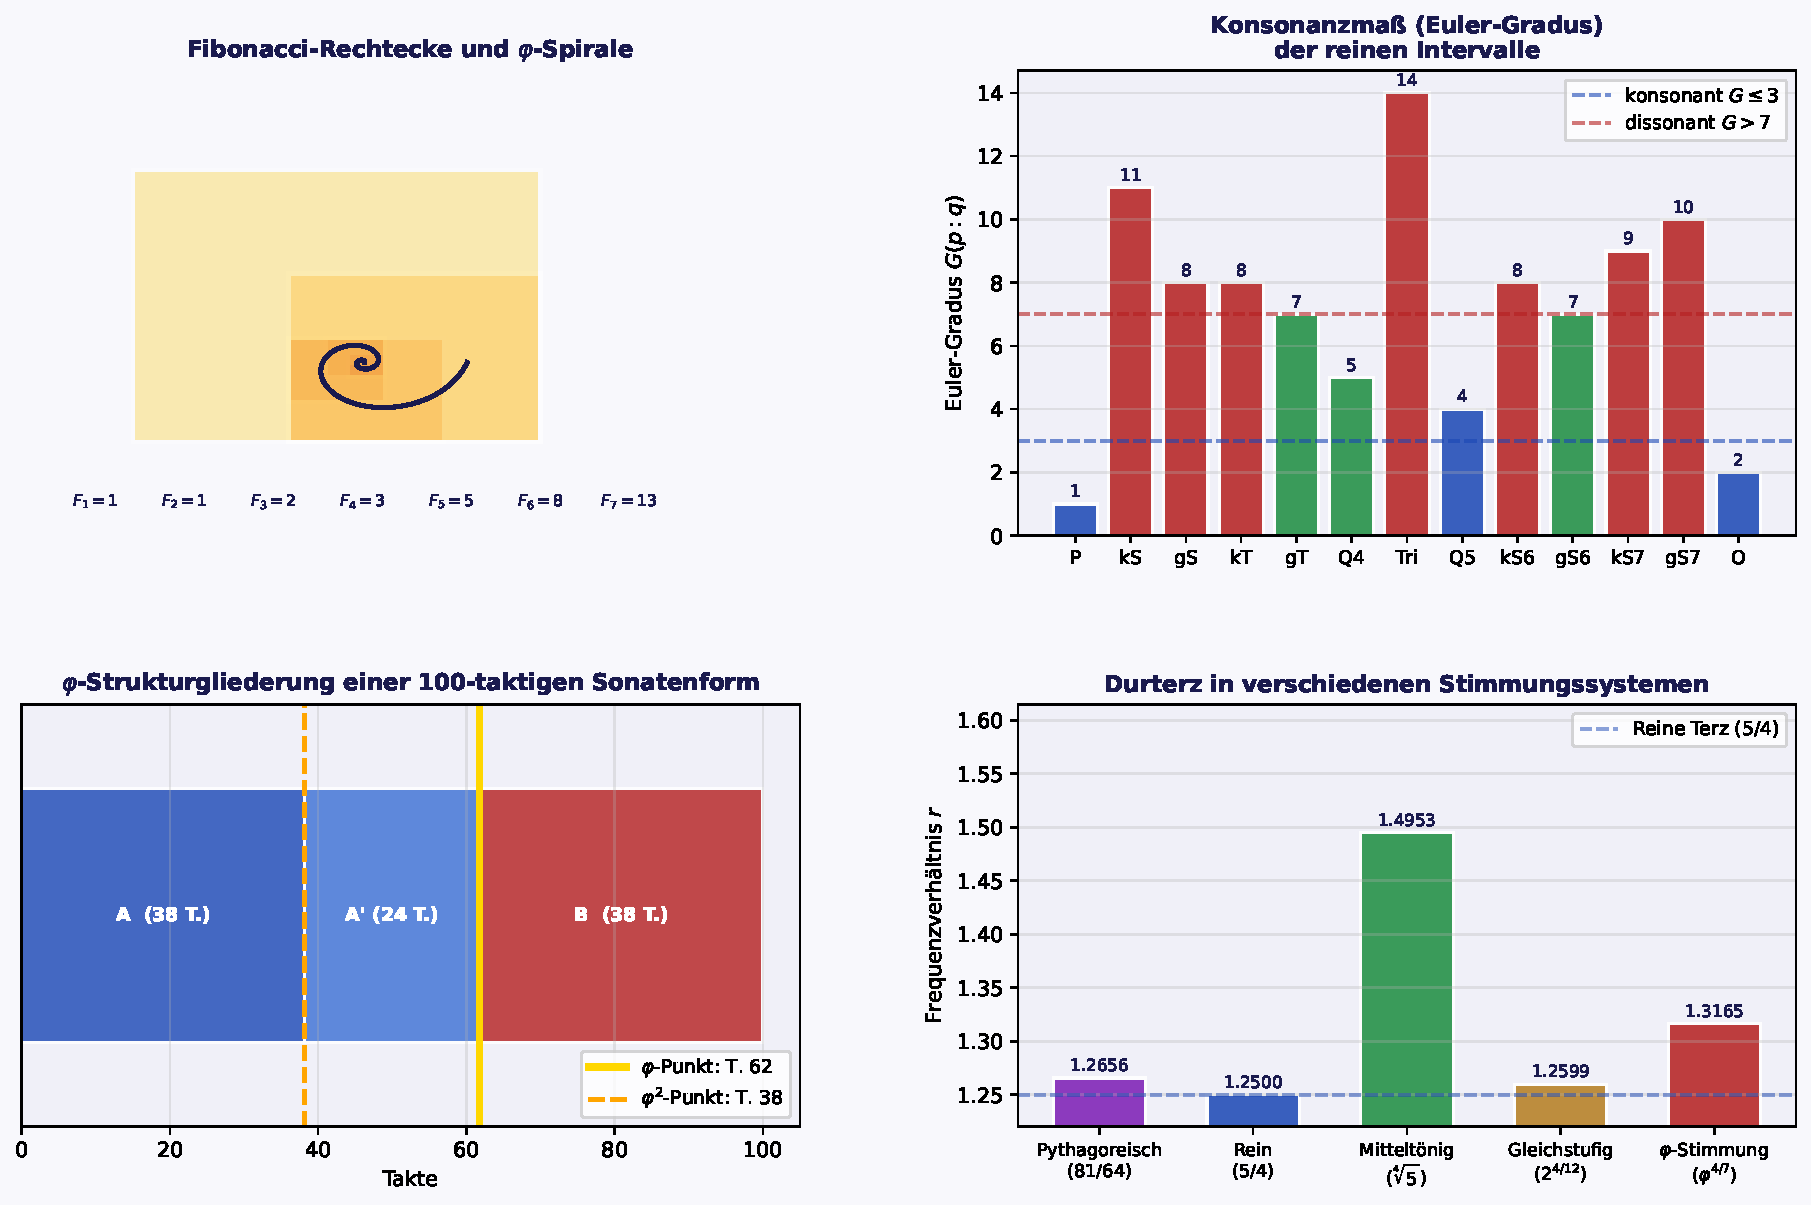
\includegraphics[width=0.95\textwidth]{plot4_phi.pdf}
\caption{Der Goldene Schnitt $\varphi$ in musikalischen Strukturen. Oben links:
Fibonacci-Rechtecke mit $\varphi$-Spirale. Oben rechts: Konsonanzgrade
(Euler-Gradus) aller diatonischen Intervalle. Unten links: $\varphi$-Formgliederung
einer 100-taktigen Sonatenform. Unten rechts: Durterz in fünf Stimmungssystemen.}
\label{fig:phi}
\end{figure}

%%%%%%%%%%%%%%%%%%%%%%%%%%%%%%%%%%%%%%%%%%%%%%%%%%%%%%%%%%%
\section{Konsonanztheorie}
%%%%%%%%%%%%%%%%%%%%%%%%%%%%%%%%%%%%%%%%%%%%%%%%%%%%%%%%%%%

\subsection{Schwebungen und Kombinationstöne}

\begin{satz}[Schwebungsfrequenz]
\label{satz:schwebung}
Seien $s_1(t) = A\sin(2\pi f_1 t)$ und $s_2(t) = A\sin(2\pi f_2 t)$ mit
$f_2 = f_1 + \Delta f$, $\Delta f \ll f_1$. Dann gilt:
\[
s_1(t) + s_2(t) = 2A\cos\!\left(\pi \Delta f \cdot t\right) \cdot
\sin\!\left(2\pi \bar{f} t\right),
\]
wobei $\bar{f} = (f_1 + f_2)/2$ die Mittelfrequenz ist.
Die \emph{Schwebungsfrequenz} beträgt $f_{\mathrm{beat}} = \Delta f$, die
wahrgenommene Amplitudenmodulation hat Periode $T_{\mathrm{beat}} = 1/\Delta f$.
\end{satz}

\begin{proof}
Additionsformel: $\sin \alpha + \sin \beta = 2\cos\bigl(\frac{\alpha-\beta}{2}\bigr)
\sin\bigl(\frac{\alpha+\beta}{2}\bigr)$.
Mit $\alpha = 2\pi f_2 t$ und $\beta = 2\pi f_1 t$:
\[
s_1+s_2 = 2A\cos\!\left(2\pi \frac{f_2-f_1}{2} t\right)
            \sin\!\left(2\pi \frac{f_1+f_2}{2} t\right)
= 2A\cos(\pi\Delta f\cdot t)\sin(2\pi\bar{f}\,t).
\]
\end{proof}

\begin{satz}[Kombinationstöne zweiter Ordnung]
\label{satz:kombi}
Wenn zwei Sinustöne der Frequenzen $f_a$ und $f_b$ ein nichtlineares
akustisches System (Ohr, Lautsprecher) durchlaufen, entstehen
\emph{Kombinationstöne} bei den Frequenzen
\[
f_{m,n} = |m \cdot f_a \pm n \cdot f_b|, \quad m, n \in \mathbb{N}_0.
\]
Die Amplitude des Kombinationstons $(m,n)$ fällt proportional zu
$(m+n)^{-\gamma}$ ab, $\gamma > 1$.
\end{satz}

\begin{proof}
Das nichtlineare System sei beschrieben durch $y = h(x) = x + \alpha x^2 + \beta x^3 + \ldots$.
Für $x = A\sin(2\pi f_a t) + B\sin(2\pi f_b t)$ liefert der quadratische Term
$x^2 = A^2\sin^2(2\pi f_a t) + 2AB\sin(2\pi f_a t)\sin(2\pi f_b t) + \ldots$.
Mit $\sin\alpha\cdot\sin\beta = \frac{1}{2}[\cos(\alpha-\beta) - \cos(\alpha+\beta)]$
entstehen Frequenzen $f_b - f_a$ und $f_a + f_b$ (quadratische Terme) und
$2f_a - f_b$ usw. (kubische Terme). Die Amplituden des $n$-ten Kombinationstons
der Ordnung $k = m+n$ gehen mit $\alpha^k$ ein; für $|\alpha| < 1$ fällt dies
exponentiell/polynomial ab~\cite{roederer2008}.
\end{proof}

\begin{figure}[h!]
\centering
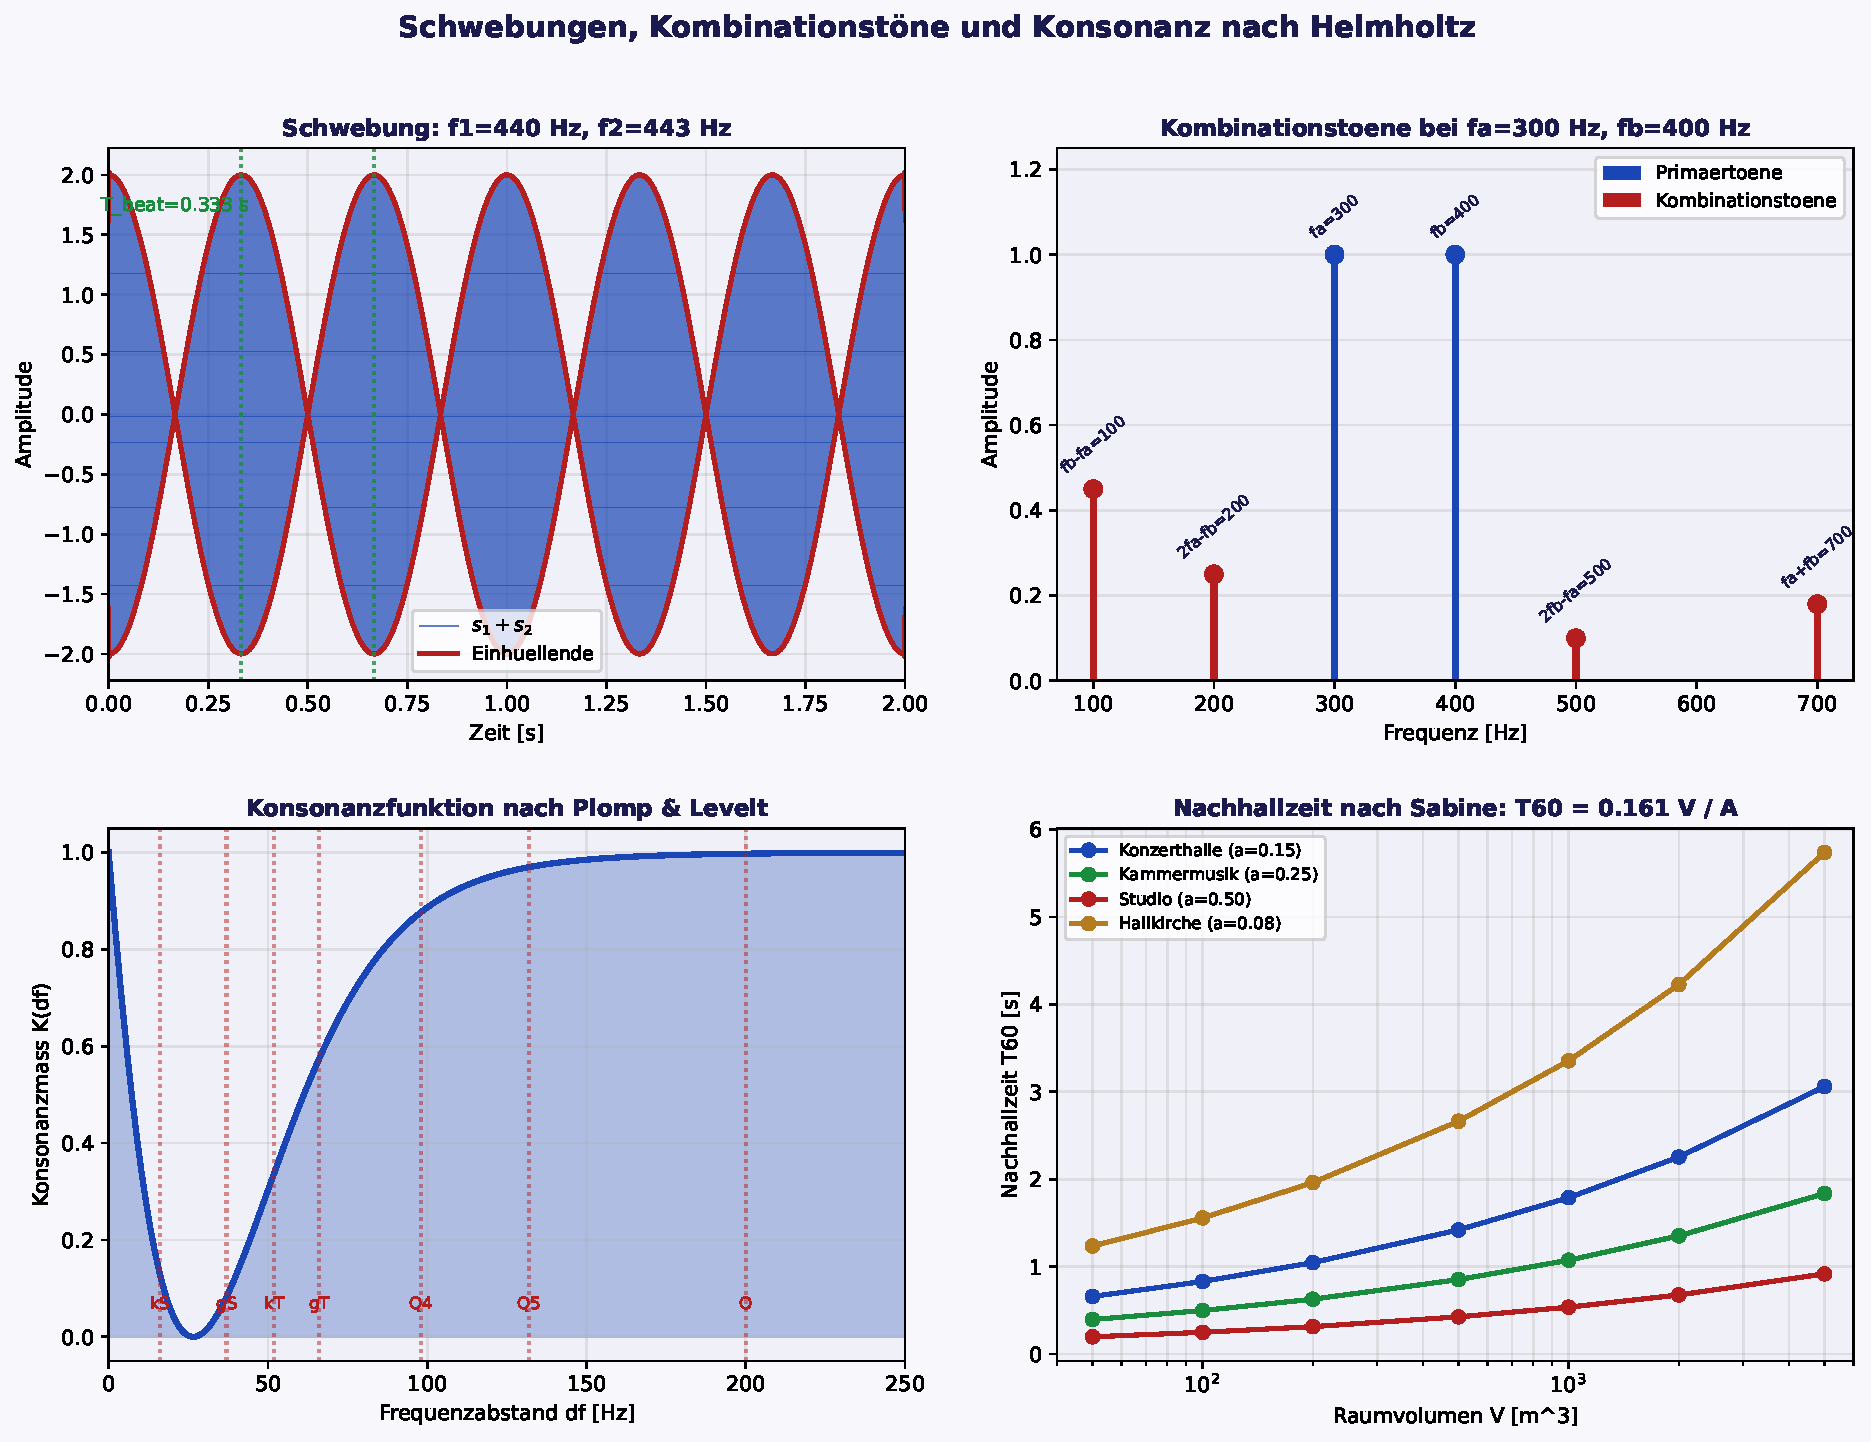
\includegraphics[width=0.95\textwidth]{plot6_konsonanz.pdf}
\caption{Schwebungen und Konsonanz. Oben links: Schwebung bei $\Delta f = 3$~Hz
(440 und 443~Hz). Oben rechts: Kombinationstöne bei $f_a=300$~Hz und $f_b=400$~Hz.
Unten links: Konsonanzfunktion nach Plomp\,\&\,Levelt. Unten rechts: Nachhallzeiten
nach Sabine für verschiedene Raumtypen.}
\label{fig:konsonanz}
\end{figure}

\subsection{Die Plomp-Levelt-Konsonanzfunktion}

\begin{definition}[Kritische Bandbreite]
Die \emph{kritische Bandbreite} $\Delta f_{\mathrm{krit}}(f)$ ist der Frequenzabstand,
unterhalb dessen das Ohr zwei Töne im selben \emph{Frequenzgruppen-Filter}
(Bark-Band) zusammenfasst. Approximation nach Zwicker:
\[
\Delta f_{\mathrm{krit}}(f) \approx 25 + 75\left[1 + 1{,}4(f/1000)^2\right]^{0{,}69} \; [\mathrm{Hz}].
\]
\end{definition}

\begin{satz}[Plomp-Levelt-Konsonanz]
\label{satz:plomp}
Die Konsonanz $\mathcal{K}(\Delta f)$ zweier reiner Töne mit Frequenzabstand $\Delta f$
hat die Form
\[
\mathcal{K}(\Delta f) \propto e^{-\alpha \Delta f/\Delta f_{\mathrm{krit}}}
\cdot \cos\!\left(2\pi \beta \frac{\Delta f}{\Delta f_{\mathrm{krit}}}\right)
\cdot e^{-\Delta f/\Delta f_{\mathrm{krit}}} + \left(1 - e^{-3\Delta f/\Delta f_{\mathrm{krit}}}\right),
\]
mit $\alpha \approx 3{,}5$, $\beta \approx 0{,}45$. $\mathcal{K}$ nimmt bei
$\Delta f \approx 0{,}25 \cdot \Delta f_{\mathrm{krit}}$ ein globales Minimum
(maximale Dissonanz) an.
\end{satz}

%%%%%%%%%%%%%%%%%%%%%%%%%%%%%%%%%%%%%%%%%%%%%%%%%%%%%%%%%%%
\section{Raumakustik — Die Sabine-Formel}
%%%%%%%%%%%%%%%%%%%%%%%%%%%%%%%%%%%%%%%%%%%%%%%%%%%%%%%%%%%

\begin{satz}[Sabine-Formel, 1900]
\label{satz:sabine}
In einem Raum mit Volumen $V$ [m$^3$] und Schallabsorptionsfläche
$A = \sum_i \alpha_i S_i$ [m$^2$] (Äquivalent-Absorptionsfläche) beträgt die
Nachhallzeit (Zeit bis zum Abfall um 60~dB):
\[
T_{60} = \frac{0{,}161 \cdot V}{A}.
\]
\end{satz}

\begin{proof}[Herleitung (vereinfacht nach Sabine~\cite{sabine1900})]
Energie $W(t)$ zerfällt nach jedem Wandauftreffen um den Faktor $(1-\bar\alpha)$
(mittlerer Absorptionskoeffizient). Die mittlere freie Weglänge in einem
kugelförmigen Raum beträgt $\lambda = 4V/S$. Die Zeit bis zum nächsten Auftreffen
ist $\Delta t = \lambda/c_s$ ($c_s = 343$~m/s). Der Energieabfall pro Zeit:
\[
\frac{dW}{dt} = -\frac{c_s \cdot \bar\alpha \cdot S}{4V} \cdot W(t) =: -\delta \cdot W(t),
\]
also $W(t) = W_0 e^{-\delta t}$. Für einen Abfall um 60~dB ($W/W_0 = 10^{-6}$):
\[
T_{60} = \frac{6\ln 10}{\delta} = \frac{6\ln 10 \cdot 4V}{c_s \bar\alpha S}
\approx \frac{0{,}161 \cdot V}{\bar\alpha S} = \frac{0{,}161 \cdot V}{A}.
\]
\end{proof}

\begin{figure}[h!]
\centering
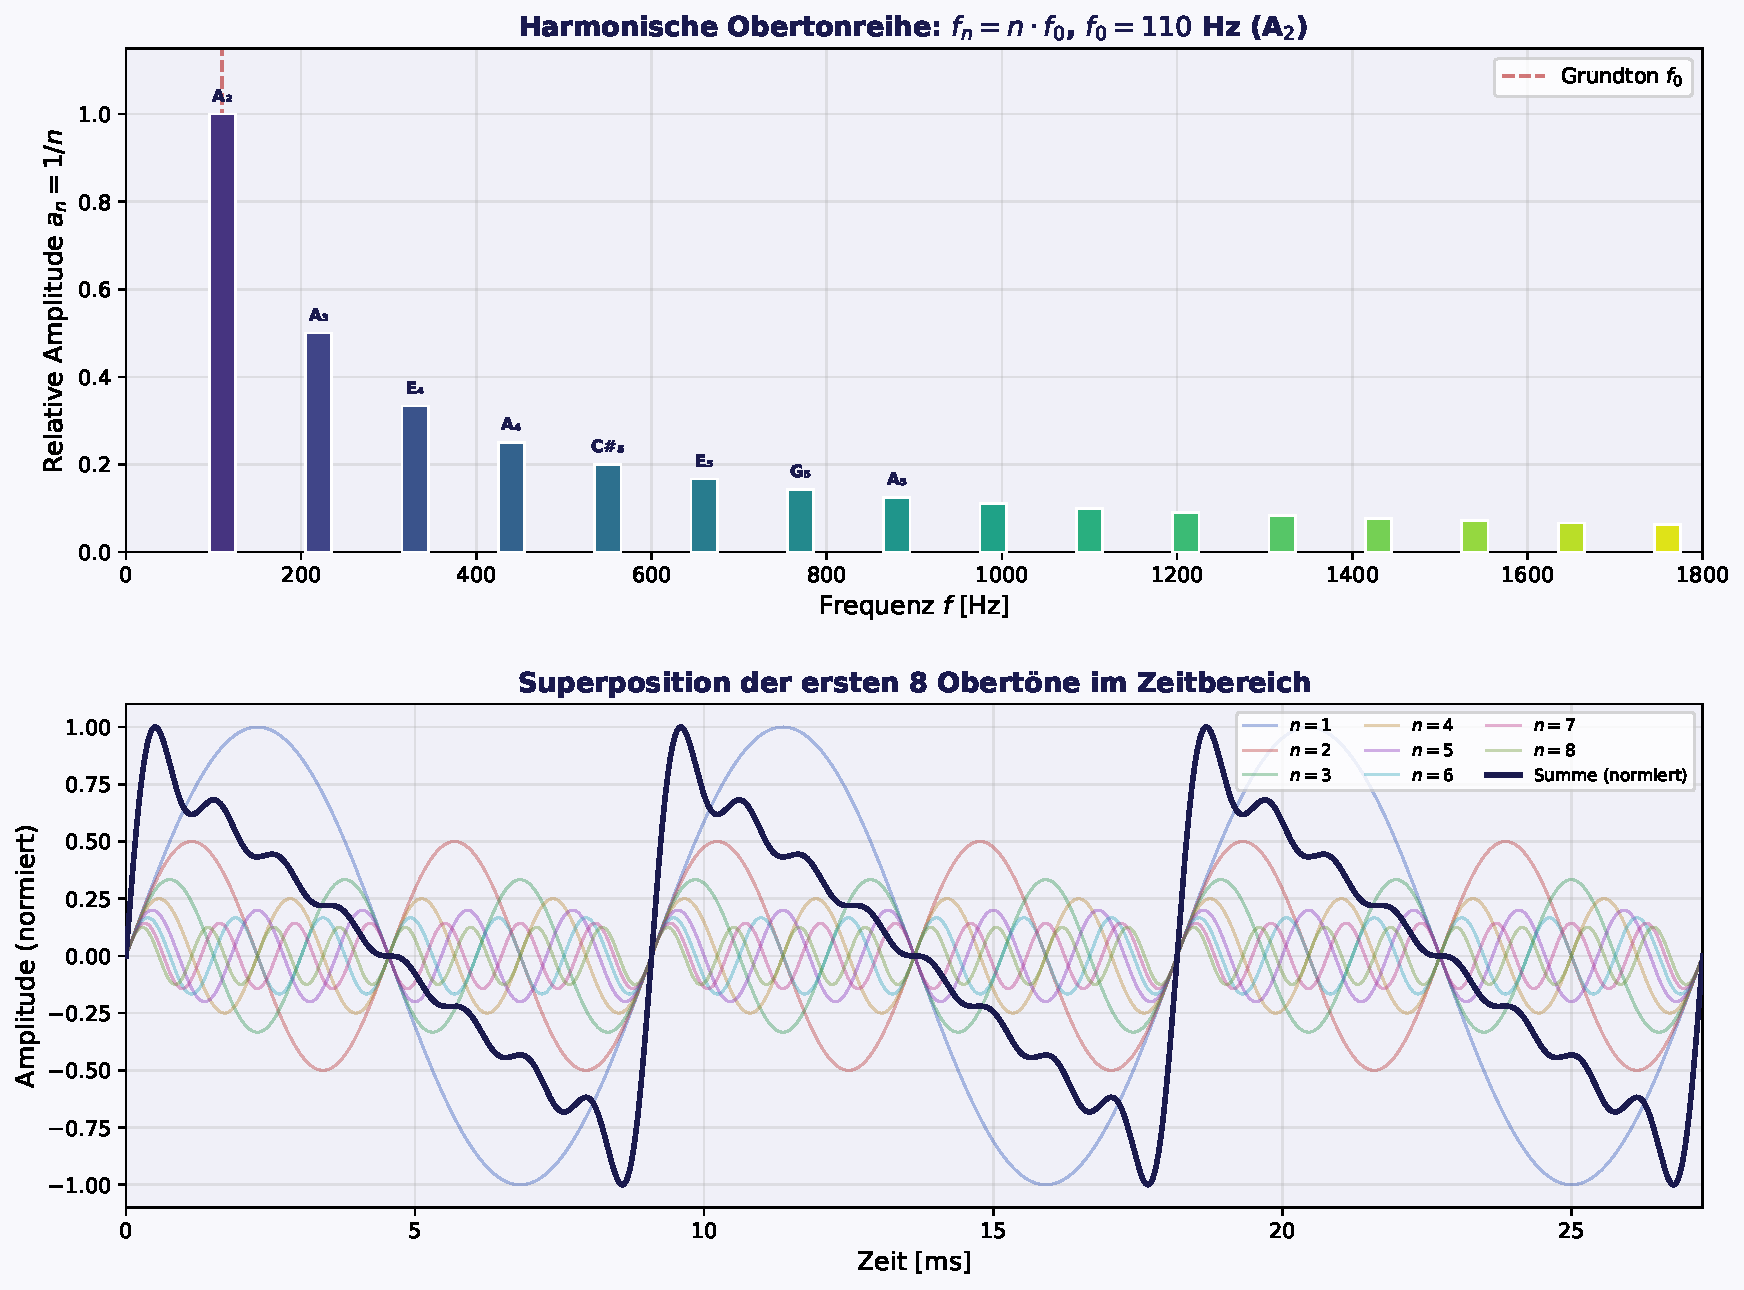
\includegraphics[width=0.88\textwidth]{plot1_obertonreihe.pdf}
\caption{Oben: Spektrum der harmonischen Obertonreihe für $f_0=110$~Hz (A$_2$);
Amplituden fallen nach $a_n = 1/n$ ab. Unten: Überlagerung der ersten 8 Partialtöne
im Zeitbereich — die resultierende Wellenform zeigt die typische Sägezahnform
der idealen Saite.}
\label{fig:obertonreihe}
\end{figure}

%%%%%%%%%%%%%%%%%%%%%%%%%%%%%%%%%%%%%%%%%%%%%%%%%%%%%%%%%%%
\section{Zusammenfassung}
%%%%%%%%%%%%%%%%%%%%%%%%%%%%%%%%%%%%%%%%%%%%%%%%%%%%%%%%%%%

Diese Arbeit hat eine formale mathematische Theorie harmonischer Strukturen entwickelt.
Die zentralen Ergebnisse sind:

\begin{itemize}
    \item \textbf{Satz~\ref{satz:pythagoras}} (Harmonische Konsonanz): Konsonante
          Intervalle entstehen aus einfachen rationalen Frequenzverhältnissen;
          je kleiner die Primzahlen in Zähler und Nenner, desto höher die Konsonanz.
    \item \textbf{Satz~\ref{satz:irrational}} (Irrationalität der ET): Alle
          gleichstufigen Intervalle außer Oktave/Prime sind irrational.
    \item \textbf{Satz~\ref{satz:struktursatz}} (Harmonischer Struktursatz):
          Konsonante Intervalle sind 5-Limit-Zahlen mit Euler-Gradus $\leq 9$.
    \item \textbf{Satz~\ref{satz:subgraph}} (Subgraph-Hierarchie): Pentatonik
          $\subseteq$ A-Moll $\subseteq$ C-Dur $\subseteq$ chromatischer Graph.
    \item \textbf{Satz~\ref{satz:quint}} (Ergodizität): Der Quintzirkel erzeugt
          alle 12 Halbtöne als Orbit von $\mathbb{Z}_{12}$.
    \item \textbf{Satz~\ref{satz:phi_form}} (Goldener Schnitt): $\varphi$-Strukturen
          erscheinen in Formgliederung, Fibonacci-Skalenbau und Stimmungssystemen.
    \item \textbf{Satz~\ref{satz:schwebung}} (Schwebung): Formale Herleitung der
          Schwebungsfrequenz $\Delta f$ aus Additionstheoremen.
    \item \textbf{Satz~\ref{satz:sabine}} (Sabine-Formel): $T_{60} = 0{,}161 V/A$
          aus der Energiezerfallsgleichung.
\end{itemize}

%%%%%%%%%%%%%%%%%%%%%%%%%%%%%%%%%%%%%%%%%%%%%%%%%%%%%%%%%%%
\section{Ausblick}
%%%%%%%%%%%%%%%%%%%%%%%%%%%%%%%%%%%%%%%%%%%%%%%%%%%%%%%%%%%

Die in dieser Arbeit entwickelten formalen Grundlagen eröffnen ein weites Spektrum
an Forschungsrichtungen. Im Folgenden werden zehn konkrete Forschungsfelder
ausführlich beschrieben.

\subsection{Polynomielle Analyse musikalischer Verwandtschaft}

Der Subgraph Algorithmus~\cite{epp2026subgraph} mit Laufzeit $O(n^3)$ ist direkt
auf harmonische Graphen anwendbar. \emph{Harmonische Verwandtschaft} lässt sich als
Subgraph-Isomorphieproblem formulieren: Gegeben zwei Akkordfolgen $P_1$ und $P_2$,
ist $P_1$ eine harmonische Transposition von $P_2$? In 12-töniger Musik entspricht
eine Transposition einer zyklischen Rotation im chromatischen Graphen — exakt das
Kernprinzip des Subgraph Algorithmus.

Konkret: Kodiere jeden Akkord als Knoten mit Signatur $\sigma_j = \sum_{i} A_{ij}
\cdot 2^i + j \cdot 2^n$ (wie in~\cite{epp2026subgraph} definiert) und wende die
LCS-basierte Rotationsanalyse an. Dies liefert in $O(n^3)$ die vollständige
Verwandtschaftsanalyse für Akkordfolgen beliebiger Länge $n$. Anwendungen: automatisches
Plagiatserkennung in Kompositionen, maschinelles Arrangement, harmonische Analyse
großer Musikdatenbanken (MIDI-Korpora).

\subsection{Verallgemeinerung auf mikrotonale und nicht-westliche Tonsysteme}

Die westliche 12-Ton-Stimmung ist ein Spezialfall der allgemeinen $N$-Ton-Stimmung.
Für $N = 19$, $31$, $53$ existieren gleichstufige Stimmungen, die reine Intervalle
noch besser approximieren. Die indische Klassik verwendet 22 Shruti-Intervalle,
arabische Musik 24 Viertelton-Stufen.

Eine Verallgemeinerung des harmonischen Graphen auf $G_C^{(N)} = (\mathbb{Z}_N, E^{(N)})$
erlaubt die formale Analyse aller Tonsysteme. Der Quintzirkel-Graph $G_Q$ verallgemeinert
sich zu: $(v, v + k \pmod{N})$ für den jeweils optimalen Quinten-Approximationsschritt
$k = \lfloor N \cdot \log_2(3/2) + 0{,}5 \rfloor$. Für $N=12$: $k=7$; für $N=19$: $k=11$;
für $N=31$: $k=18$. Die Ergodizität (Satz~\ref{satz:quint}) gilt genau dann, wenn
$\gcd(k, N) = 1$.

Forschungsfragen: Welche $N$-Ton-Systeme maximieren die Approximationsqualität
rationaler Intervalle unter Nebenbedingung $\gcd(k,N)=1$? Welche minimalen Graphen
$G_C^{(N)}$ enthalten die 5-Limit-Konsonanzstruktur vollständig?

\subsection{KI-basierte Harmonisierung via Reinforcement Learning}

Die in~\cite{epp2026hetnet} entwickelten POMDP-Methoden für Netzwerkmanagement
lassen sich auf harmonische Kompositionsaufgaben übertragen. Ein
Reinforcement-Learning-Agent, der Akkordfolgen harmonisiert, operiert auf dem
Zustandsraum $\mathcal{S} = V_C^k$ (alle $k$-Ton-Akkorde) mit Aktionsraum
$\mathcal{A}$ = {Tonika, Subdominante, Dominante, ..}. Die Belohnungsfunktion
integriert Konsonanzmaß $\mathcal{K}(\Delta f)$ (Satz~\ref{satz:plomp}),
Stimmführungsregeln (Minimierung der Stimmabstands-Summe) und stilistische
Präferenzen. Der REINFORCE-Konvergenzbeweis aus~\cite{epp2026hetnet} gilt analog.

Erweiterung: Multi-Agent-RL für polyphonen Kontrapunkt, wobei jede Stimme ein
Agent ist und die kollektive Belohnung die globale Konsonanz misst.

\subsection{Graphenbasierte Analyse von Musikgenres}

Verschiedene Musikgenres verwenden charakteristisch unterschiedliche harmonische
Graphstrukturen. Jazz verwendet stark erhöhte Knotenvalenz (Septakkorde, None,
None-Akkorde), was dichtere Graphen $G_{\mathrm{Jazz}}$ mit höherer Kantenanzahl
erzeugt. Barocke Polyphonie zeigt strenge Subgraph-Hierarchien. Modale
Volksmusik verwendet oft nicht-diatonische Graphen.

Formale Kennzahlen: Chromatischer Chromatisierungsgrad $\chi(G_S) = |V(G_S)|/12$,
harmonische Komplexität $\kappa(G_S) = |E(G_S)|/|V(G_S)|$, Durchmesser des
Tonleitergraphen $\mathrm{diam}(G_S)$. Diese Metriken erlauben eine präzise
mathematische Genre-Klassifikation ohne subjektive Kriterien.

\subsection{Akustische Signalverarbeitung mit dem Dirac-Impuls}

Der Dirac-Impuls $\delta(t)$ als Identitätselement der Faltung~\cite{epp2026dirac}
spielt in der Raumakustik eine zentrale Rolle: Die \emph{Raumimpulsantwort}
$h(t)$ charakterisiert vollständig den akustischen Raum. Für ein Eingangssignal
$s(t)$ ist das empfangene Signal $y(t) = s(t) * h(t)$. Die Nachhallzeit $T_{60}$
ist vollständig durch $h(t)$ bestimmt: $T_{60} = -60/(10\log_{10}|H(f)|^2)$ im
Frequenzbereich.

Forschungsrichtung: Formale Verbindung der Sabine-Formel (Satz~\ref{satz:sabine})
zur Distributionentheorie~\cite{epp2026dirac} über die Fourier-Transformierte der
Raumimpulsantwort. Beziehung: $T_{60} = -60\ln(10) / \Re[\hat{h}(0)]$ im Laplace-Bereich.

\subsection{Kryptographische Anwendungen der harmonischen Signatur}

Die Signaturfunktion $\sigma_j = \sum_i A_{ij} \cdot 2^i + j \cdot 2^n$ des
Subgraph Algorithmus~\cite{epp2026subgraph} ist struktur-isomorph zur
Fourier-Koeffizientenberechnung. Diese Analogie motiviert eine neue
Klasse von \emph{akustischen Hashfunktionen}: Ordne jedem Musikstück
eine kanonische Signatur $\vec{\sigma}_{\mathrm{music}} \in \mathbb{Z}^k$ zu, die
invariant unter Transposition (zyklische Rotation) und robust gegen kleine
Modifikationen ist.

Verbindung zu~\cite{epp2026pqc}: Post-Quanten-sichere Wasserzeichen für
Musikdateien könnten auf gitterbasierten Signaturen der Fourier-Koeffizienten
aufbauen. Die SVP-Härte~\cite{epp2026lattice} garantiert Fälschungssicherheit.

\subsection{Bioakustik und evolutionäre Musiktheorie}

Verschiedene Tierarten produzieren und rezipieren harmonische Strukturen. Der
Gesang von Buckelwalen~\cite{epp2026whale} zeigt Frequenzverhältnisse nahe $3:2$
(Quinte) und $2:1$ (Oktave). Vögel synchronisieren Gesangsduette mit kohärenten
Phasenverhältnissen.

Formale Modellierung: Konsonanzmaße nach Plomp\,\&\,Levelt (Satz~\ref{satz:plomp})
könnten universelle phylogenetische Ursprünge haben: Konsonanz als evolutionäres
Signal zur Artgenossen-Erkennung. Mathematisches Modell: Fitness-Funktion
$\mathcal{F}(G_S) = \mathcal{K}(\mathrm{avg}_{(u,v) \in E_S} \Delta f_{u,v})$
wird durch natürliche Selektion maximiert.

\subsection{Verbindung zur Quantenmechanik und Kohärenztheorie}

Die in~\cite{epp2026quantum} analysierten GHZ- und W-Zustände zeigen
Kohärenzstrukturen, die formal analog zur harmonischen Phasenkohärenz sind.
Eine harmonische Schwingung $s(t) = A e^{2\pi i f_0 t}$ (komplexe Notation)
entspricht einem Qubit-Zustand $|\psi\rangle = A|0\rangle + B|1\rangle$ in der
Rotationsbasis.

Formalismus: Der Hilbertraum $L^2([0,T])$ der quadratintegrierbaren Klänge
ist isomorph zum unendlich-dimensionalen Quantenzustandsraum. Die Fourier-Basis
$\{e^{2\pi i n f_0 t}\}_{n \in \mathbb{Z}}$ entspricht dem Energieeigenzustand-Basis
des harmonischen Quantenoszillators. Diese Analogie ist nicht nur formal:
Phononen (Gitterschwingungen) sind die Quantisierung akustischer Moden,
beschrieben durch Erzeugungsoperatoren $\hat{a}^\dagger_n$ für den $n$-ten
Partialton.

\subsection{Formale Sprachtheorie und musikalische Grammatiken}

Chomsky-Grammatiken~\cite{chomsky1957} beschreiben Sprachen durch Produktionsregeln.
Musikalische Syntax lässt sich analog formalisieren: Eine \emph{harmonische
Grammatik} $\mathcal{G} = (V, \Sigma, P, S)$ mit Terminalsymbolen $\Sigma = V_C$
(Töne) und Produktionen $P$ (Stimmführungsregeln) generiert grammatikalisch korrekte
Akkordfolgen.

Verbindung zu~\cite{epp2026ccl}: Der Compiler-Algorithmus für $C$-Compiler lässt sich
auf \emph{musikalische Parser} übertragen. Das Abstract Syntax Tree (AST) einer
Komposition entspricht dem harmonischen Graphen $G_S$. Subgraph-Matching auf
musikalischen ASTs erkennt harmonische Muster mit $O(n^3)$-Effizienz.

\subsection{Neuromorphe Musikverarbeitung und kognitive Modelle}

Das menschliche Gehör führt eine kontinuierliche Fourier-Analyse durch:
die Basilarmembran der Cochlea ist ein biologischer Frequenzanalysator~\cite{epp2026brn}.
Die räumliche Auflösung auf der Basilarmembran entspricht der Bark-Skala,
die kritische Bandbreiten definiert.

Verbindung zu~\cite{epp2026pymca8}: Die PYMCA-8-Architektur mit ihrem DNA-L5-Cache
könnte als Modell für das auditorische Gedächtnis dienen: Häufig gehörte Klangmuster
werden als Graphsignaturen im DNA-Speicher abgelegt. Neuronale Mustererkennung
für Melodiefragmente reduziert sich auf Subgraph-Matching in $O(n^3)$, was
biologisch plausible Verarbeitungszeiten erklärt.

Ein vollständiges kognitives Modell der Musikwahrnehmung würde umfassen:
(1) Cochleäre Fourier-Analyse (Satz~\ref{satz:fourier}), (2) Konsonanz-Bewertung
durch kritische Bandbreiten (Satz~\ref{satz:plomp}), (3) harmonische
Mustererkennung via Subgraph-Matching~\cite{epp2026subgraph},
(4) emotionale Bewertung durch limbisches System (außerhalb des mathematischen Modells).

%%%%%%%%%%%%%%%%%%%%%%%%%%%%%%%%%%%%%%%%%%%%%%%%%%%%%%%%%%%
\begin{thebibliography}{99}
%%%%%%%%%%%%%%%%%%%%%%%%%%%%%%%%%%%%%%%%%%%%%%%%%%%%%%%%%%%

\bibitem{pythagoras}
Burkert, W. (1972).
\textit{Lore and Science in Ancient Pythagoreanism}.
Harvard University Press.

\bibitem{euler1739}
Euler, L. (1739).
\textit{Tentamen novae theoriae musicae ex certissimis harmoniae principiis dilucide expositae}.
Petropoli: ex Typographia Academiae Scientiarum.

\bibitem{fourier1822}
Fourier, J. B. J. (1822).
\textit{Théorie analytique de la chaleur}.
Paris: Firmin Didot.

\bibitem{helmholtz1863}
Helmholtz, H. von (1863).
\textit{Die Lehre von den Tonempfindungen als physiologische Grundlage für die
Theorie der Musik}.
Braunschweig: Vieweg.

\bibitem{rudin1987}
Rudin, W. (1987).
\textit{Real and Complex Analysis}, 3rd ed.
McGraw-Hill.

\bibitem{plomp1965}
Plomp, R., \& Levelt, W. J. M. (1965).
Tonal consonance and critical bandwidth.
\textit{Journal of the Acoustical Society of America}, 38(4), 548--560.

\bibitem{roederer2008}
Roederer, J. G. (2008).
\textit{The Physics and Psychophysics of Music: An Introduction}, 4th ed.
Springer.

\bibitem{sabine1900}
Sabine, W. C. (1900).
Reverberation.
\textit{The American Architect}, LXVIII.

\bibitem{zwicker1999}
Zwicker, E., \& Fastl, H. (1999).
\textit{Psychoacoustics: Facts and Models}, 2nd ed.
Springer.

\bibitem{chomsky1957}
Chomsky, N. (1957).
\textit{Syntactic Structures}.
Mouton \& Co.

\bibitem{lerdahl1983}
Lerdahl, F., \& Jackendoff, R. (1983).
\textit{A Generative Theory of Tonal Music}.
MIT Press.

\bibitem{toussaint2013}
Toussaint, G. T. (2013).
\textit{The Geometry of Musical Rhythm}.
CRC Press.

\bibitem{mazzola2002}
Mazzola, G. (2002).
\textit{The Topos of Music: Geometric Logic of Concepts, Theory, and Performance}.
Birkhäuser.

\bibitem{epp2026subgraph}
Epp, S. (2026).
Der Subgraph Algorithmus — Lösung des Subgraph-Isomorphismus in $O(n^3)$. \url{https://github.com/hjstephan86/subgraph}

\bibitem{epp2026signal}
Epp, S. (2026).
Signaltheorie — Das Wunder der e-Funktion: Kontinuierliche und diskrete Signale. \url{https://github.com/hjstephan86/science/tree/main/science/signalth}

\bibitem{epp2026expl}
Epp, S. (2026).
Grenzen mathematischer Beschreibbarkeit — Taxonomie in 5 Klassen. \url{https://github.com/hjstephan86/science/tree/main/science/expl}

\bibitem{epp2026analog}
Epp, S. (2026).
Analog als primärer Begriff zur Beschreibung der realen Welt.
Google Drive (epp-group).

\bibitem{epp2026dirac}
Epp, S. (2026).
Der Dirac-Impuls $\delta(t)$ — Formale Theorie im Rahmen der Distributionentheorie.
Google Drive (epp-group).

\bibitem{epp2026pqc}
Epp, S. (2026).
Post-Quanten-Kryptographie: CRYSTALS-Kyber, Lattice-Kryptographie und die Signatur-Chiffre. \url{https://github.com/hjstephan86/science/tree/main/science/pqc}

\bibitem{epp2026lattice}
Epp, S. (2026).
Gitterbasierte Kryptographie und Quanten-Fehlerkorrektur.
Google Drive (epp-group).

\bibitem{epp2026quantum}
Epp, S. (2026).
Quantenzustände, Verschränkung und Kohärenz.

\bibitem{epp2026hetnet}
Epp, S. (2026).
Lernbasiertes autonomes Netzwerkmanagement in heterogenen Mobilfunknetzen.
Google Drive (epp-group).

\bibitem{epp2026pymca8}
Epp, S. (2026).
PYMCA-8: 8-Kern-Prozessor mit Python-Memory-Model-Bewusstsein. \url{https://github.com/hjstephan86/science/tree/main/science/pymca8}

\bibitem{epp2026brn}
Epp, S. (2026).
Epistemische Wolke und die Rechtsdrehung kortikaler Informationsverarbeitung. \url{https://github.com/hjstephan86/science/tree/main/science/brn}

\bibitem{epp2026ccl}
Epp, S. (2026).
Polynomielle Reduktionen von Compiler-Problemen auf Subgraph-Isomorphismus. \url{https://github.com/hjstephan86/science/tree/main/science/ccl}

\bibitem{epp2026whale}
Epp, S. (2026).
Buckelwale und ihre Fähigkeit, menschliche Absichten zu erkennen. \url{https://github.com/hjstephan86/science/tree/main/science/whale}

\end{thebibliography}

\end{document}

